\chapter{Abstraction and Structure}
\label{chap:V_abstraction}

In the previous chapters it became clear
that laws of nature\index{law of nature}
are not described by intuitive images,
but by mathematical relationships.
Motion\index{motion},
growth\index{growth},
and dynamics\index{dynamics}
can be understood only
when change\index{change}
is expressed formally.
This raises a further question:
How is it possible
that abstract mathematical concepts
capture real natural phenomena so precisely?

The answer lies in the principle of abstraction\index{abstraction}.
Mathematics\index{mathematics}
deliberately leaves aside many properties of reality
in order to uncover its structural features.
It does not describe
\emph{what} an object is materially,
but \emph{how} it behaves
and in which relationships it stands to other objects.
Abstraction is therefore not a loss of reality\index{reality},
but a deliberate reduction to what is essential.

Structure\index{structure}
refers precisely to what remains under this reduction.
It is independent of concrete material,
scale,
or position\index{position}.
Whether a system consists of points,
particles\index{particle},
or fields\index{field}
is initially secondary for the mathematical structure.
What matters is only the network of relationships
that connects these elements with one another.

This chapter examines
how abstraction and structure work together
and why they are indispensable
for understanding modern mathematics
and physics\index{physics}.
It shows
that mathematics is successful not because it copies reality,
but because it uncovers its structures.

% =====================================================
% 5.1 Vectors and Spaces
% =====================================================
\subsection{Vectors and Spaces}

The concept of the vector\index{vector}
is one of the best-known elements of mathematics\index{mathematics}
and physics\index{physics}.
In school contexts, it usually appears as an arrow
with direction, length, and orientation.
This image is intuitive and useful,
but it does not capture the true core.
A vector is not primarily a geometric picture,
but an abstract element of a space\index{space}.

This shift in perspective is decisive.
Mathematics is not interested in
what a vector looks like,
but in how it relates to other vectors.
Addition\index{addition},
scaling\index{scaling},
and comparison are not merely calculation procedures,
but expressions of an underlying structure.
Only through such relationships
is a space mathematically determined.

A space is therefore not simply a set of points\index{point}.
It is a system of relations\index{relation}
in which certain operations are meaningfully defined.
Which objects form this space
is initially secondary.
Vectors can represent displacements\index{displacement} in space,
velocities\index{velocity},
forces\index{force},
states\index{state},
or abstract informational content.
What matters is not their particular interpretation,
but the structure\index{structure}
they have in common.

Here the power of abstraction\index{abstraction}
becomes especially clear.
By disregarding the concrete interpretation,
mathematics makes very different phenomena comparable.
One and the same vector space\index{vector space}
can describe motions,
structure electric fields\index{field},
or represent states in quantum mechanics\index{quantum mechanics}.
What changes
is the physical meaning --
not the mathematical form.

This point of view reverses the usual way of thinking.
The space is not fixed by intuitive images;
rather, the elements receive their meaning
through the space in which they lie.
A vector is therefore not ``in itself'' an arrow,
but becomes what it is mathematically
only through the structure of the space.
Here abstraction does not mean renunciation,
but precision.

The introduction of vector spaces therefore marks a turning point.
Mathematics detaches itself from intuitive individual forms
and formulates relationships
that are valid independently of dimension\index{dimension},
scale,
or physical context.
A space can be finite- or infinite-dimensional,
continuous or discrete --
the formal relationships remain the same.

This makes understandable
why modern physics\index{modern physics}
cannot do without such abstract spaces.
Fields are not mere collections of numbers,
but elements of suitable function spaces\index{function space}.
Quantum states are not trajectories,
but vectors in abstract state spaces\index{state space}.
Reality\index{reality}
is thereby described not more visually,
but more relationally.

Vectors and spaces are therefore not merely technical aids,
but fundamental tools of thought.
They show, in exemplary fashion,
how mathematics does not simply depict reality,
but grasps its order structurally.
Abstraction is not the removal of reality here,
but the condition for being able
to recognize its form at all.

A simple example makes this point of view intuitive.
Let us consider a two-dimensional space\index{two-dimensional space},
as familiar from the plane.
A vector is often represented there as an arrow
pointing from one point to another.
What matters, however, is not its concrete position,
but its effect as a displacement.

If such an arrow is shifted in parallel
without changing its direction or length,
it remains mathematically the same vector.
Its meaning lies not in the starting point,
but in the relationship between start and end.
Precisely this independence from position\index{position}
characterizes the abstract concept of a vector.

This becomes especially clear in the graphical representation:

\begin{center}
	\begin{tikzpicture}[scale=1.1]
		
		% Coordinate axes
		\draw[->] (-0.5,0) -- (4.5,0) node[right] {$x$};
		\draw[->] (0,-0.5) -- (0,3.5) node[above] {$y$};
		
		% First vector
		\draw[thick,->] (0.5,0.5) -- (2.5,1.5);
		
		% Second (shifted) vector
		\draw[thick,->] (1.0,2.0) -- (3.0,3.0);
		
	\end{tikzpicture}
\end{center}

Both arrows represent the same vector,
although they are drawn at different positions.
For mathematics, only the displacement is relevant,
not its embedding at a particular point of the plane.
The space provides the framework
in which such relations are meaningfully defined.

This simple example shows the core of abstraction:
the geometric drawing serves only as an illustration.
The true object of mathematics
is the structure
common to all possible representations.
Vectors are not arrows in space --
they are elements of a space
defined by its relationships.

% =====================================================
% 5.2 Symmetries and Invariance
% =====================================================

\subsection{Symmetries and Invariance}

After vectors\index{vector}
have been introduced as elements of abstract spaces\index{space},
a further question arises:
How can one recognize the structure\index{structure} of such a space?
The answer lies not in individual objects,
but in what \emph{does not} change
under transformations\index{change}.
This is precisely where the concept of symmetry\index{symmetry} begins.

In everyday language,
symmetry is often associated with mirror images
or aesthetic balance.
In mathematics\index{mathematics}
and physics\index{physics},
however, the term has a more precise meaning.
A symmetry is present
when an object or a system
remains unchanged under a certain transformation.
What matters is not the transformation itself,
but what remains invariant\index{invariance}.

This idea can be generalized easily.
A displacement\index{displacement} in space
changes the position of a body,
but not its shape.
A rotation\index{rotation}
changes the orientation,
but not the distances between points\index{point}.
In both cases, certain properties are preserved.
Precisely these preserved properties
reveal the underlying structure.

In physics, such invariances play a central role.
Laws of nature\index{law of nature}
are characterized by the fact
that they hold independently of position\index{position},
time\index{time},
or orientation.
Whether an experiment is carried out here or there,
whether it takes place today or tomorrow,
whether the coordinate system\index{coordinate system} is rotated --
the law remains the same.
This independence is no accident,
but the expression of a deep symmetry of nature.

\begin{DidacticBox}[What Symmetry Means]
	\phantomsection\label{box:symmetry}
	Symmetry does not describe uniformity,
	but preservation.
	A system is symmetric
	when certain properties remain unchanged under transformations.
	
	What matters is not the transformation,
	but what \emph{does not} change.
\end{DidacticBox}

Mathematically, this idea
is made precise by transformations\index{transformation}.
A transformation is an allowed change of a system --
for example a displacement,
rotation,
or reflection\index{reflection}.
If a certain property is preserved under this transformation,
one speaks of invariance.
Symmetries are therefore not geometric games,
but statements about structural stability\index{stability}.

This point of view is fundamental
for understanding modern physics\index{modern physics}.
Conserved quantities\index{conserved quantity}
such as energy\index{energy},
momentum\index{momentum},
or angular momentum\index{angular momentum}
are not isolated postulates,
but consequences of symmetries.
They do not arise from individual measurements,
but from the structure of the underlying laws.
Mathematics makes these connections visible
even before a concrete experiment is considered.

It is remarkable
that symmetries are independent
of the particular carrier material.
They apply equally to particles\index{particle},
fields\index{field},
or abstract state spaces\index{state space}.
What changes
is the interpretation --
not the structure.
Symmetry is therefore
a universal organizing principle\index{organizing principle}
that extends far beyond intuitive geometry.

From this perspective, it becomes clear
why abstraction\index{abstraction} is necessary.
Only the renunciation of concrete images
makes it possible
to uncover the invariant properties of a system.
Mathematics does not describe
what a system looks like,
but which transformations it allows
without losing its essence.

Symmetries and invariance
therefore form a central building block
of modern descriptions of nature.
They connect abstract spaces
with physical reality\index{reality}
and show
that the order of nature
lies less in its appearances
than in the relationships\index{relation}
that connect these appearances with one another.

A simple example illustrates
the connection between symmetry and invariance.
Let us consider a physical system
that moves along a straight line.
If we shift the entire system
by a fixed distance,
the positions involved change,
but not the underlying law of motion\index{law of motion}.

For physics, what matters is
that the law holds independently of the chosen reference point\index{reference frame}.
Whether the motion begins at one place
or at another
does not matter.
The displacement changes the description,
but not the structure of the law.
This independence
is called translational invariance\index{translational invariance}.

Both representations therefore describe the same physical law,
although the systems are located at different positions.
The displacement changes the coordinates\index{coordinate},
but not the relationships between the quantities involved.
The law remains invariant under translation\index{translation}.

\begin{center}
	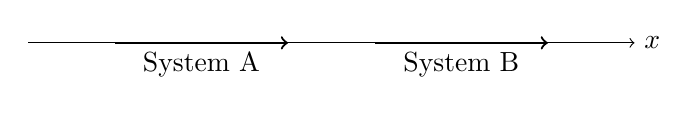
\begin{tikzpicture}[scale=1.1]
		
		% Axis
		\draw[->] (-0.5,0) -- (6.5,0) node[right] {$x$};
		
		% First system
		\draw[thick,->] (0.5,0) -- (2.5,0);
		\node[below] at (1.5,0) {System A};
		
		% Second (shifted) system
		\draw[thick,->] (3.5,0) -- (5.5,0);
		\node[below] at (4.5,0) {System B};
		
	\end{tikzpicture}
\end{center}

This example shows the core of the symmetry idea:
a law of nature is fundamental precisely when
it holds independently of arbitrary choices
such as position,
time,
or orientation.
Symmetries are therefore not additional assumptions,
but a test
of the general validity of physical laws.

% =====================================================
% 5.3 Mathematics as a Universal Structural Principle
% =====================================================
\subsection{Mathematics as a Universal Structural Principle}

The preceding considerations show
that mathematics\index{mathematics}
does not work with individual things,
but with structures\index{structure}.
Precisely for this reason,
the same mathematical form
can recur in very different areas of nature\index{nature}.

What appears in mechanics\index{mechanics}
as a law of motion
can reappear in electrodynamics\index{electrodynamics},
in quantum physics\index{quantum physics},
or in field theory\index{field theory}
in a new form.
The objects described differ,
but the underlying relationships remain comparable.
What differs is the meaning,
not the form.

This is the universality of mathematics\index{universality}.
It does not describe the material composition of things,
but the patterns
that different systems have in common.
When different phenomena
follow the same structural laws,
they necessarily appear in the same mathematical language.

This universality is no accident
and not merely the result of human convention.
It follows from the way
mathematics works:
through abstraction,
through relations,
and through uncovering invariant connections.
Precisely for this reason, it can reach
beyond individual domains
and become the general structural principle
of the description of nature.

Mathematics is therefore not only a tool
with which known phenomena are ordered.
It also shows
which forms can even be considered
as generally valid descriptions.
What is structurally unstable or mathematically inconsistent
cannot claim fundamental status.

This makes understandable
why mathematics speaks the same language
in such different areas:
not because the phenomena are the same,
but because their structures are related.
Precisely in this structural kinship
lies its universality.

% =====================================================
% 5.4 Abstraction as a Path to Reality
% =====================================================

\subsection{Abstraction as a Path to Reality}

In everyday language,
abstraction\index{abstraction}
is often regarded as the opposite of reality\index{reality}.
What is abstract
seems distant,
theoretical,
or artificial.
In mathematics\index{mathematics}
and physics\index{physics},
however, abstraction means something fundamentally different.
It is not a removal from reality,
but a deliberate filtering out of what is essential
for understanding.

Even simple physical models\index{model}
operate abstractly.
A body is treated as a point\index{point},
friction\index{friction} is neglected,
and ideal conditions\index{idealization} are assumed.
Such simplifications are not deceptions,
but deliberate choices.
They make structures\index{structure} visible
that would otherwise remain hidden
in the complexity of real situations.

Abstraction acts like a magnifying glass.
By suppressing secondary effects,
the fundamental relationships\index{relation}
stand out more clearly.
A model is useful not because
it contains everything,
but because it leaves out exactly the right things.
Reality is not copied,
but uncovered in its order.

\begin{DidacticBox}[Abstraction and Reality]
	\phantomsection\label{box:abstraction}
	Abstraction does not mean loss of reality.
	It means focus.
	
	What is left out
	are context-dependent properties.
	What remains
	is the underlying structure.
\end{DidacticBox}

Modern physics\index{modern physics}
in particular shows the necessity of this approach.
Quantum mechanics\index{quantum mechanics},
relativity theory\index{relativity theory},
and field theories\index{field theory}
operate with concepts
that elude immediate intuition.
Nevertheless, they deliver the most precise predictions\index{prediction}
known in physics.
Their closeness to reality
is not shown in pictures,
but in the accuracy of their statements.

This development is no accident.
The deeper one penetrates into the structure of nature\index{nature},
the less intuitive images can carry the explanation.
Abstract concepts replace concrete images
because they remain invariant\index{invariance}
under different representations.
Mathematics makes precisely these invariant structures visible
and detaches them from subjective perception\index{perception}.

Abstraction is therefore not a detour,
but the direct path to reality.
It makes it possible
to recognize general lawful relationships\index{law of nature}
that go beyond individual observations.
What at first seems distant
turns out, on closer inspection,
to be the most reliable thing
we can say about nature.

In this sense, abstraction forms
both the conclusion and the transition of this chapter.
It connects the mathematical language of nature
with its structural order
and opens the view onto those domains
in which structure becomes visible not only in deterministic laws,
but also in probability\index{probability},
chance\index{chance},
and uncertainty\index{uncertainty}.
There, too, mathematics remains
not the opposite of reality,
but its most precise means of expression.

\subsection*{Transition: Structure and Chance}

The preceding considerations have shown
that mathematics displays its strength precisely where
it looks beyond the surface of appearances
and uncovers the underlying structure.
But this raises a new and more difficult question:
What happens
when the world appears to us not as ordered,
but as random?

Not all phenomena follow simple,
deterministic paths.
Throws, decays, fluctuations, and unpredictable events
seem to evade the claim of strict lawfulness.
Precisely here it becomes clear
how far mathematical description actually reaches.
Is chance a feature of the world itself --
or only a sign
that our description has reached its limits?

Thus the question of abstraction and structure
leads directly to the next problem:
the role of chance,
probability,
and uncertainty in our understanding of reality.